\apendice
\chapter{ANÁLISE BIBLIOMÉTRICA}

A bibliometria foi realizada por meio do levantamento bibliográfico relacionado ao tema da pesquisa, utilizando o mecanismo de busca Google Acadêmico, e as bases de periódicos da CAPES, \textit{SCOPUS} e \textit{ScienceDirect}. As principais expressões de busca utilizadas foram: ``project management'' , ``project management agile'', ``agile'' e a tradução destas para a língua portuguesa. A seguir será apresentado os passos desta análise.

\section{Material não disponibilizado pela base CAPES}

O levantamento bibliográfico das fontes impressas e digitais, que não se encontravam disponiveis pela Portal Capes, foi realizado através do portal \textit{ScienceDirect} e do mecanismo Google Acadêmico, que dispõe de bancos de teses e dissertações de instituições específicas, e aprensenta redirecionamento às bases Biblioteca Digital Brasileira de Teses e Dissertações (BDTD), Scientific Electronic Library Online (SciELO).

Ressalta-se ainda que o mecanismo de busca Google Acadêmico também indexa em suas pesquisas as bases de periódicos da CAPES, \textit{SCOPUS} e \textit{ScienceDirect}, permitindo ao usuário avaliar a relevância de citações de um determinado periódico em ambas as bases, e redirecionando o usuário as bases para leitura dos períodicos.

Foi realizada também, uma pesquisa sobre o tema para saber sobre o interesse no mesmo nos ultímos anos, para tanto foi utilizada a ferramenta Google \textit{Trends}. Primeiramente foi utilizada a frase de pesquisa ``project management'' para demonstrar o interesse específico sobre as práticas de GP. O resultado apresentado no gráfico \ref{trends1}, que parte do ano de 2006, declinando em pesquisas até o ano de 2016.


\begin{figure}[!ht]
  \centering
  \scalebox{0.5}{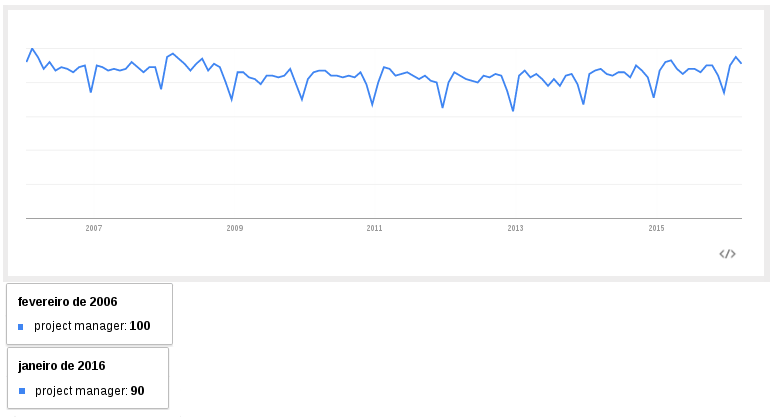
\includegraphics{figuras/trends1}}
  \caption{Interesse sobre práticas de GP ao passar do tempo. Fonte: Google \textit{Trends} (2016).}
  \label{trends1}
\end{figure}


Para saber o interesse sobre práticas de GP que fossem consideradas agéis foi somada a pesquisa a frase ``project management agile'', para que assim pudesse haver um comparação sobre o interesse dessas práticas com o passar do tempo. O resultado desta pesquisa é apontado no gráfico \ref{trends2}, onde o interesse pela gestão de projetos apresenta um declinío lento, enquanto o interesse pela gestão ágil de projetos cresce, também lentamente.

\begin{figure}[!ht]
  \centering
  \scalebox{0.5}{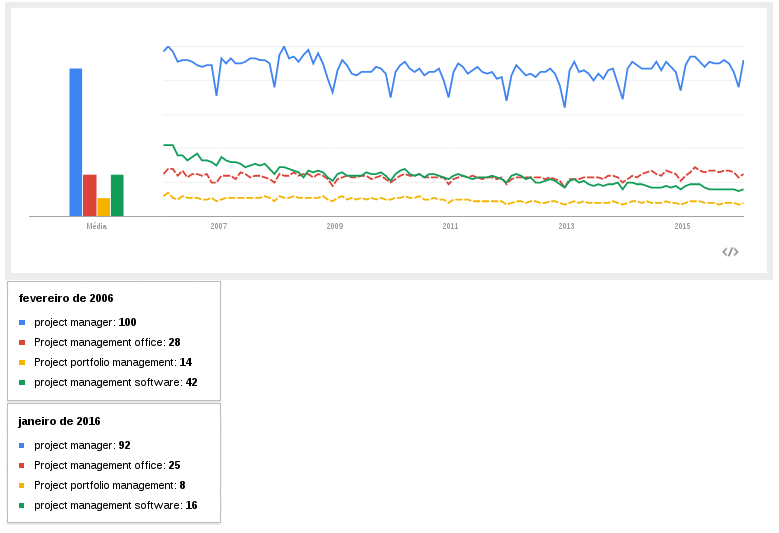
\includegraphics{figuras/trends2}}
  \caption{Interesse sobre práticas de GP versus práticas agéis ao passar do tempo. Fonte: Google \textit{Trends} (2016).}
  \label{trends2}
\end{figure}


Os indicadores bibliométricos escolhidos foram os seguintes: ano de publicação, idiomas, autores e tipos de documento. Seguindo os indicadores escolhidos, a seleção dos artigos foi feita considerando os seguintes critérios:

\begin{itemize}
  \item \textbf{Ano de Publicação:} foi considerado o periodo de 2005 a 2015, isto é, a equivalências aos ultimos dez anos, pois entende-se que este periodo compreende os anos de maior interesse no tema de pesquisa de acordo com mecanismo utilizado.
  \item \textbf{Idiomas:} foi dada preferência ao inglês pela importancia que os períodicos desse idioma representaram, entretanto também foram escolhidos períodicos em português pela sua relevância ao tema proposto.
  \item \textbf{Autores:} foram consideradas principalmente publicações de autores mais pesquisados e mais citados.
  \item \textbf{Tipos de Documento:} foi dada preferência a publicações em periodicos, por traduzirem pensamentos mais recentes relativos ao tema de pesquisa.
\end{itemize}


Os trabalhos selecionados a partir da análise bibliometrica, após a aplicação dos indicadores mencionados, encontram-se relacionados no quadro \ref{tabela_autores}.

\begin{longtable}{| p{.20\textwidth} | p{.80\textwidth} |}
  \cline{1-2}
  \cellcolor[HTML]{C0C0C0}{\color[HTML]{000000} Autor(es)} & \cellcolor[HTML]{C0C0C0}{\color[HTML]{000000} Publicação} \\ \hline
  ALMEIDA, L. F. M. et al. & Fatores críticos da agilidade no gerenciamento de projetos de desenvolvimento de novos produtos (2012) \\ \hline
  AMARAL, D. C. et al. & Gerenciamento ágil de projetos: aplicação em produtos inovadores (2011). \\ \hline
  ATKINSON, R. D.; EZELL, S. J.; STEWART, L. A. & The global innovation policy index(2012). \\ \hline
  BARLOW, J. B. et al. & Overview and guidance on agile development in large organizations(2011). \\ \hline
  BATRA, D. et al. & Balancing agile and structured development approaches to successfully manage large distributed software projects: A case study from the cruise line industry(2010). \\ \hline
  BECK, K. et al. & Manifesto for agile software development(2001). \\ \hline
  BERGGREN, C.; SÖDERLUND, J. & Rethinking project management education: Social twists and knowledge co-production(2008). \\ \hline
  BINDER, J.; AILLAUD, L. I.; SCHILLI, L. & The project management cocktail model: An approach for balancing agile and iso 21500(2014). \\ \hline
  BOEHM, B.; TURNER, R. & Management challenges to implementing agile processes in traditional development organizations(2005). \\ \hline
  CAMPBELL, D. F.; GUTTEL, W. H. & Knowledge production of firms: research networks and the"scientification"of business r\&d(2005). \\ \hline
  CICMIL, S. J. et al. & Exploring the complexity of projects: Implications of complexity theory for project management practice(2009). \\ \hline
  COCKBURN, A. & Agile software development(2006). \\ \hline
  COLLYER, S. et al. & Aim, fire, aim—project planning styles in dynamic environments(2010). \\ \hline
  CONFORTO, E. C.; AMARAL, D. C. & Evaluating an agile method for planning and controlling innovative projects(2010). \\ \hline
  ETZKOWITZ, H.; KLOFSTEN, M. & The innovating region: toward a theory of knowledge-based regional development(2005). \\ \hline
  FERNANDEZ, D. J.; FERNANDEZ, J. D. & Agile project management—agilism versus traditional approaches(2008). \\ \hline
  GANGULY, A.; NILCHIANI, R.; FARR, J. V. & Evaluating agility in corporate enterprises(2009). \\ \hline
  GERALDI, J. G. et al. & Innovation in project management: Voices of researchers(2008). \\ \hline
  HASS, K. B. & The blending of traditional and agile project management(2007). \\ \hline
  HIGHSMITH, J.; COCKBURN, A. & Agile software development: The business of innovation(2009). \\ \hline
  KOLLTVEIT, B. J.; KARLSEN, J. T.; GRØNHAUG, K. & Perspectives on project management(2007). \\ \hline
  LASTRES, H. M.; CASSIOLATO, J. E.; ARROIO, A. & Conhecimento, sistemas de inovação e desenvolvimento(2005). \\ \hline
  LEYBOURNE, S. A. & Improvisation and agile project management: a comparative consideration(2009). \\ \hline
  MIR, F. A.; PINNINGTON, A. H. & Exploring the value of project management: linking project management performance and project success(2014). \\ \hline
  QUMER, A.; HENDERSON-SELLERS, B. & An evaluation of the degree of agility in six agile methods and its applicability for method engineering(2010). \\ \hline
  STARE, A. & Agile project management in product development projects(2014). \\ \hline
  STYHRE, A. & The bureaucratization of the project manager function: The case of the construction industry(2006). \\ \hline
  WILLIAMS, T. & Assessing and moving on from the dominant project management discourse in the light of project overruns(2005). \\ \hline
  WINTER, M. et al. & Directions for future research in project management: The main findings of a uk government-funded research network(2006). \\ \hline
  \caption{Publicações Selecionadas. Autoria própria (2016).}
  \label{tabela_autores}
\end{longtable}
